\section{Introduction}

Home and gym fitness applications increasingly employ AI-based pose estimation to count exercise repetitions, yet most still lack real-time, adaptive coaching on movement quality.
Early research systems such as Pose Trainer~\cite{chen2020pose} and AIFit~\cite{fieraru2021aifit} demonstrate that 3D pose analysis can detect posture errors and evaluate performance, but their pipelines remain largely offline, relying on recorded videos and computationally heavy 3D reconstruction.
As a result, these systems provide limited personalization and cannot adapt feedback dynamically during a workout.
More recent work such as ARFit~\cite{mandic2023arfit} integrates augmented-reality visualization to guide users through motion sequences, but still applies generic thresholds and lacks quantitative evaluation of performance consistency across repetitions and viewpoints.

Commercial applications (e.g., Top Pushup~\cite{toppushup}, QuickPose~\cite{quickpose}) have popularized real-time motion counting and form tracking using smartphone cameras.
However, their analysis is typically shallow, focusing on repetition detection or coarse form classification without distinguishing good versus poor repetitions, assessing tempo stability, or tracking joint-level consistency over time.
Moreover, most commercial apps rely on fixed, population-level thresholds and offer limited adaptive or personalized feedback beyond simple prompts.


\textbf{FitCoachAR} aims to bridge the gap between academic models and consumer applications by providing a \textbf{lightweight, real-time, and adaptive coaching system}.
It monitors exercises via 2D pose estimation, detects common form errors, and delivers feedback through \textbf{augmented-reality overlays} and \textbf{coach-style natural language cues}.
The system personalizes its critique level through a short calibration phase and produces both live corrections and post-session summaries.

This project addresses three major motivations:
\begin{itemize}
    \item \textbf{Accessibility}: Eliminate the dependency on motion-capture equipment, camera calibration, and high-end GPUs.
    \item \textbf{Personalization}: Adapt thresholds and critique sensitivity ($\delta$) to each user rather than relying on fixed global rules.
    \item \textbf{Interactivity}: Transform static, after-exercise evaluation into \textbf{continuous, real-time feedback} that enhances engagement and training quality.
\end{itemize}

\subsection{System Overview}
Figure~\ref{fig:system_overview} presents the system architecture. The user interacts through the interface, which captures video and displays feedback. The backend performs pose estimation, filtering, and rep counting, then passes data to the feedback engine which returns results to the interface.

\begin{figure}[ht]
\centering
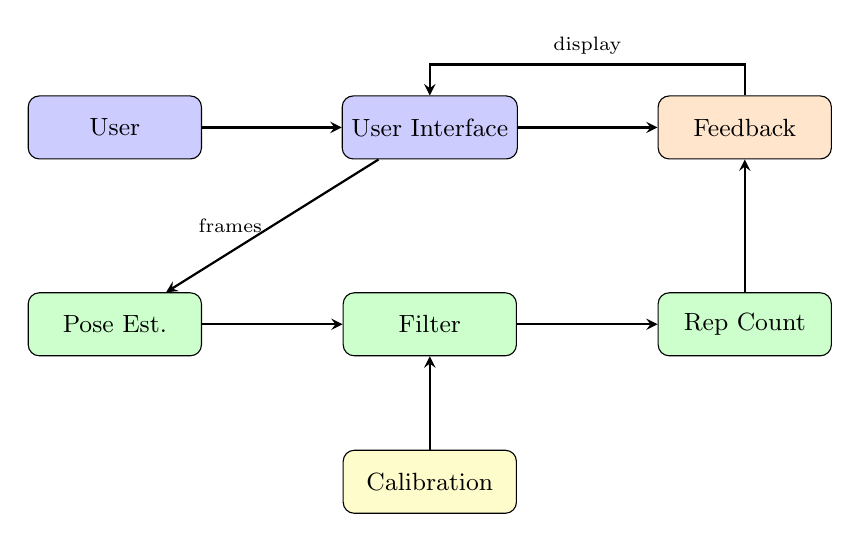
\begin{tikzpicture}[
    box/.style={rectangle, draw, rounded corners, minimum width=2.2cm, minimum height=0.8cm, align=center, font=\small},
    arrow/.style={->, >=stealth, thick}
]

% Top row: User flow
\node[box, fill=blue!20] (user) at (0,0) {User};
\node[box, fill=blue!20] (ui) at (4,0) {User Interface};
\node[box, fill=orange!20] (feedback) at (8,0) {Feedback};

% Bottom row: Processing pipeline
\node[box, fill=green!20] (pose) at (0,-2.5) {Pose Est.};
\node[box, fill=green!20] (filter) at (4,-2.5) {Filter};
\node[box, fill=green!20] (rep) at (8,-2.5) {Rep Count};

% Calibration below
\node[box, fill=yellow!20] (calib) at (4,-4.5) {Calibration};

% Arrows - top row
\draw[arrow] (user) -- (ui);
\draw[arrow] (ui) -- (feedback);
\draw[arrow] (feedback) -- ++(0,0.8) -| node[pos=0.25,above,font=\scriptsize]{display} (ui);

% Arrows - UI to processing
\draw[arrow] (ui) -- node[left,font=\scriptsize]{frames} (pose);

% Arrows - processing pipeline
\draw[arrow] (pose) -- (filter);
\draw[arrow] (filter) -- (rep);
\draw[arrow] (rep) -- (feedback);

% Calibration arrow
\draw[arrow] (calib) -- (filter);

\end{tikzpicture}
\caption{FitCoachAR system architecture.}
\label{fig:system_overview}
\end{figure}














